\documentclass[12pt]{article}

\usepackage{xcolor}
\usepackage{ amssymb, amsmath, graphicx }
\usepackage{mathtools}
 
\addtolength{\textheight}{2.7in}
\addtolength{\topmargin}{-1.15in}
\addtolength{\textwidth}{1.0in}
\addtolength{\evensidemargin}{-0.5in}
\addtolength{\oddsidemargin}{-0.65in}
\setlength{\parskip}{0.1in}
\setlength{\parindent}{0.0in}

\newcommand{\given}{\, | \,}

\pagestyle{empty}

\raggedbottom
 
\begin{document}

\vspace*{-0.3in}

\hfill
Computational Models

\begin{center}

\textbf{\large Practice}

\end{center}


1. Convert the CFG an equivalent PDA \\
\textbf{Solution:} \\
Basically turning the CFG into a stack-based PDA. \\
\vspace*{0.3in}
\centerline{ 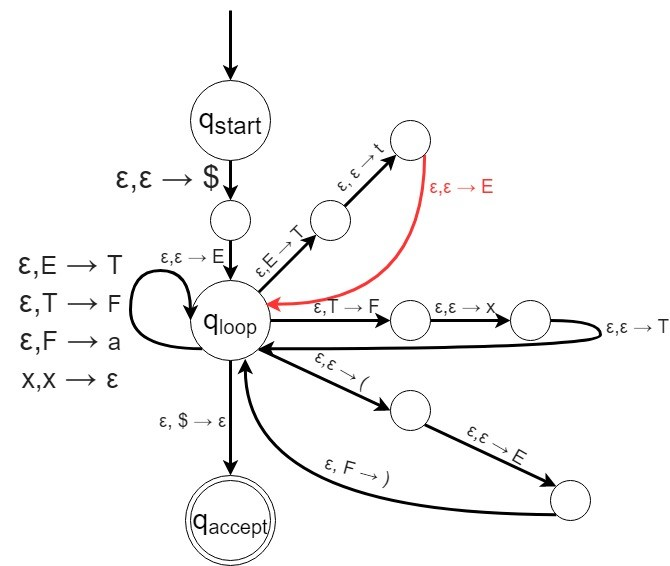
\includegraphics[scale=.85]{2.11.JPG}}

Convert the CFG $G$ given in Exercise 2.3 to an equivalent PDA, using the procedure given in Theorem 2.20. \\
\textbf{Solution:} \\
\centerline{ 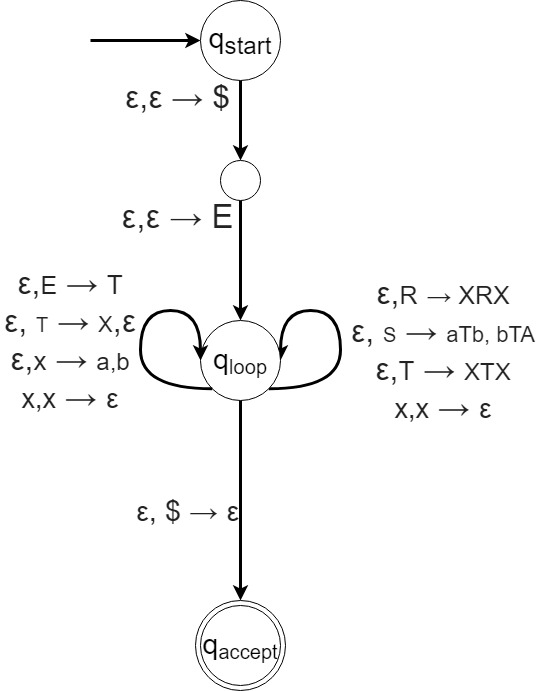
\includegraphics[scale=.65]{2.12.JPG}}

Convert the following CFG into an equivalent CFG in Chomsky normal form, using the procedure given in Theorem 2.9.
\begin{eqnarray} \nonumber
A &\to & BAB \textrm{ } | \textrm{ } B \textrm{ } | \textrm{ } \epsilon \\ \nonumber
B &\to & 00 \textrm{ } | \textrm{ } \epsilon \\  \nonumber
\end{eqnarray}
\textbf{Solution:} \\
%Note: I am adding an S-state to do CKY algorithm. 
\begin{eqnarray} \nonumber
A &\to & BAB \ | \ B \ | \ \epsilon \\ \nonumber
B &\to & 00 \ | \ \epsilon \\  \nonumber
\\ \nonumber
\textrm{Goes through B} & \textrm{and} & \textrm{adds stages to A }\\  \nonumber
\textrm{And } & \textrm{removed} & \epsilon \\ \nonumber
A &\to & BAB \ | \ BB \ | \ 00 \ | \ AB \ | \ BA \ | \\ \nonumber
B &\to & 00  \\  \nonumber
\\ \nonumber
\textrm{Added } & \textrm{C} & \\  \nonumber
A &\to & BC \ | \ BB \ | \ 00 \ | \ C \ | \ BA \ | \\ \nonumber
B &\to & 00  \\  \nonumber
C &\to & AB  \\  \nonumber
\\ \nonumber
\textrm{Added } & \textrm{D} & \\  \nonumber
A &\to & BC \ | \ BB \ | \ DD \ | \ C \ | \ BA \ | \\ \nonumber
B &\to & DD  \\  \nonumber
C &\to & AB  \\  \nonumber
D &\to & 0  \\  \nonumber
\\ \nonumber
\end{eqnarray}

\end{document}
